% Options for packages loaded elsewhere
\PassOptionsToPackage{unicode}{hyperref}
\PassOptionsToPackage{hyphens}{url}
\PassOptionsToPackage{dvipsnames,svgnames,x11names}{xcolor}
%
\documentclass[
]{article}

\usepackage{amsmath,amssymb}
\usepackage{setspace}
\usepackage{iftex}
\ifPDFTeX
  \usepackage[T1]{fontenc}
  \usepackage[utf8]{inputenc}
  \usepackage{textcomp} % provide euro and other symbols
\else % if luatex or xetex
  \usepackage{unicode-math}
  \defaultfontfeatures{Scale=MatchLowercase}
  \defaultfontfeatures[\rmfamily]{Ligatures=TeX,Scale=1}
\fi
\usepackage{lmodern}
\ifPDFTeX\else  
    % xetex/luatex font selection
\fi
% Use upquote if available, for straight quotes in verbatim environments
\IfFileExists{upquote.sty}{\usepackage{upquote}}{}
\IfFileExists{microtype.sty}{% use microtype if available
  \usepackage[]{microtype}
  \UseMicrotypeSet[protrusion]{basicmath} % disable protrusion for tt fonts
}{}
\makeatletter
\@ifundefined{KOMAClassName}{% if non-KOMA class
  \IfFileExists{parskip.sty}{%
    \usepackage{parskip}
  }{% else
    \setlength{\parindent}{0pt}
    \setlength{\parskip}{6pt plus 2pt minus 1pt}}
}{% if KOMA class
  \KOMAoptions{parskip=half}}
\makeatother
\usepackage{xcolor}
\usepackage[left=1in,right=1in,top=1.1in,bottom=1.1in,heightrounded]{geometry}
\setlength{\emergencystretch}{3em} % prevent overfull lines
\setcounter{secnumdepth}{5}
% Make \paragraph and \subparagraph free-standing
\makeatletter
\ifx\paragraph\undefined\else
  \let\oldparagraph\paragraph
  \renewcommand{\paragraph}{
    \@ifstar
      \xxxParagraphStar
      \xxxParagraphNoStar
  }
  \newcommand{\xxxParagraphStar}[1]{\oldparagraph*{#1}\mbox{}}
  \newcommand{\xxxParagraphNoStar}[1]{\oldparagraph{#1}\mbox{}}
\fi
\ifx\subparagraph\undefined\else
  \let\oldsubparagraph\subparagraph
  \renewcommand{\subparagraph}{
    \@ifstar
      \xxxSubParagraphStar
      \xxxSubParagraphNoStar
  }
  \newcommand{\xxxSubParagraphStar}[1]{\oldsubparagraph*{#1}\mbox{}}
  \newcommand{\xxxSubParagraphNoStar}[1]{\oldsubparagraph{#1}\mbox{}}
\fi
\makeatother


\providecommand{\tightlist}{%
  \setlength{\itemsep}{0pt}\setlength{\parskip}{0pt}}\usepackage{longtable,booktabs,array}
\usepackage{calc} % for calculating minipage widths
% Correct order of tables after \paragraph or \subparagraph
\usepackage{etoolbox}
\makeatletter
\patchcmd\longtable{\par}{\if@noskipsec\mbox{}\fi\par}{}{}
\makeatother
% Allow footnotes in longtable head/foot
\IfFileExists{footnotehyper.sty}{\usepackage{footnotehyper}}{\usepackage{footnote}}
\makesavenoteenv{longtable}
\usepackage{graphicx}
\makeatletter
\newsavebox\pandoc@box
\newcommand*\pandocbounded[1]{% scales image to fit in text height/width
  \sbox\pandoc@box{#1}%
  \Gscale@div\@tempa{\textheight}{\dimexpr\ht\pandoc@box+\dp\pandoc@box\relax}%
  \Gscale@div\@tempb{\linewidth}{\wd\pandoc@box}%
  \ifdim\@tempb\p@<\@tempa\p@\let\@tempa\@tempb\fi% select the smaller of both
  \ifdim\@tempa\p@<\p@\scalebox{\@tempa}{\usebox\pandoc@box}%
  \else\usebox{\pandoc@box}%
  \fi%
}
% Set default figure placement to htbp
\def\fps@figure{htbp}
\makeatother
% definitions for citeproc citations
\NewDocumentCommand\citeproctext{}{}
\NewDocumentCommand\citeproc{mm}{%
  \begingroup\def\citeproctext{#2}\cite{#1}\endgroup}
\makeatletter
 % allow citations to break across lines
 \let\@cite@ofmt\@firstofone
 % avoid brackets around text for \cite:
 \def\@biblabel#1{}
 \def\@cite#1#2{{#1\if@tempswa , #2\fi}}
\makeatother
\newlength{\cslhangindent}
\setlength{\cslhangindent}{1.5em}
\newlength{\csllabelwidth}
\setlength{\csllabelwidth}{3em}
\newenvironment{CSLReferences}[2] % #1 hanging-indent, #2 entry-spacing
 {\begin{list}{}{%
  \setlength{\itemindent}{0pt}
  \setlength{\leftmargin}{0pt}
  \setlength{\parsep}{0pt}
  % turn on hanging indent if param 1 is 1
  \ifodd #1
   \setlength{\leftmargin}{\cslhangindent}
   \setlength{\itemindent}{-1\cslhangindent}
  \fi
  % set entry spacing
  \setlength{\itemsep}{#2\baselineskip}}}
 {\end{list}}
\usepackage{calc}
\newcommand{\CSLBlock}[1]{\hfill\break\parbox[t]{\linewidth}{\strut\ignorespaces#1\strut}}
\newcommand{\CSLLeftMargin}[1]{\parbox[t]{\csllabelwidth}{\strut#1\strut}}
\newcommand{\CSLRightInline}[1]{\parbox[t]{\linewidth - \csllabelwidth}{\strut#1\strut}}
\newcommand{\CSLIndent}[1]{\hspace{\cslhangindent}#1}

\usepackage{array}
\usepackage{pdfpages}
\usepackage{longtable}
\usepackage{graphicx}
\usepackage{booktabs}
\usepackage{dcolumn}
\usepackage{float}
\usepackage{array}
\usepackage{longtable}
\setlength{\parskip}{1.2em}
\usepackage{tabularx}
\makeatletter
\@ifpackageloaded{caption}{}{\usepackage{caption}}
\AtBeginDocument{%
\ifdefined\contentsname
  \renewcommand*\contentsname{Table of contents}
\else
  \newcommand\contentsname{Table of contents}
\fi
\ifdefined\listfigurename
  \renewcommand*\listfigurename{List of Figures}
\else
  \newcommand\listfigurename{List of Figures}
\fi
\ifdefined\listtablename
  \renewcommand*\listtablename{List of Tables}
\else
  \newcommand\listtablename{List of Tables}
\fi
\ifdefined\figurename
  \renewcommand*\figurename{Figure}
\else
  \newcommand\figurename{Figure}
\fi
\ifdefined\tablename
  \renewcommand*\tablename{Table}
\else
  \newcommand\tablename{Table}
\fi
}
\@ifpackageloaded{float}{}{\usepackage{float}}
\floatstyle{ruled}
\@ifundefined{c@chapter}{\newfloat{codelisting}{h}{lop}}{\newfloat{codelisting}{h}{lop}[chapter]}
\floatname{codelisting}{Listing}
\newcommand*\listoflistings{\listof{codelisting}{List of Listings}}
\makeatother
\makeatletter
\makeatother
\makeatletter
\@ifpackageloaded{caption}{}{\usepackage{caption}}
\@ifpackageloaded{subcaption}{}{\usepackage{subcaption}}
\makeatother

\usepackage{bookmark}

\IfFileExists{xurl.sty}{\usepackage{xurl}}{} % add URL line breaks if available
\urlstyle{same} % disable monospaced font for URLs
\hypersetup{
  pdftitle={SNA4DS Project - Report Submission 2},
  pdfauthor={Leon Boeren - Noud van Summeren - Chau Nguyen - Paritosh Singh - Silvia Petrova},
  colorlinks=true,
  linkcolor={blue},
  filecolor={Maroon},
  citecolor={Blue},
  urlcolor={Blue},
  pdfcreator={LaTeX via pandoc}}


\title{SNA4DS Project - Report Submission 2}
\usepackage{etoolbox}
\makeatletter
\providecommand{\subtitle}[1]{% add subtitle to \maketitle
  \apptocmd{\@title}{\par {\large #1 \par}}{}{}
}
\makeatother
\subtitle{Group 08}
\author{Leon Boeren - Noud van Summeren - Chau Nguyen - Paritosh Singh -
Silvia Petrova}
\date{2025-11-14}

\begin{document}
\maketitle

\renewcommand*\contentsname{Table of contents}
{
\hypersetup{linkcolor=}
\setcounter{tocdepth}{2}
\tableofcontents
}

\setstretch{1.28}
\newpage{}

\section*{Glossary}\label{glossary}
\addcontentsline{toc}{section}{Glossary}

\phantomsection\label{sec-gloss}
\setlength{\arrayrulewidth}{0.05pt}
\begin{longtable}{p{0.28\textwidth} p{0.68\textwidth}}
\caption{Definitions of Key Terms}
 \\
\hline
\textbf{Term} & \textbf{Definition} \\
\hline
\endfirsthead

\hline
\textbf{Term} & \textbf{Definition} \\
\hline
\endhead

\hline
\endfoot

\hline
\endlastfoot

Bilateral Trade 
&
Trade between two specific countries, measured as exports from one to the other and vice versa. \\
\hline

Export value 
&
The total monetary value of goods and services sold by one country to another, measured in U.S. dollars. \\
\hline

Macroeconomic Stability 
&
The condition in which a country experiences low inflation, steady growth, and minimal fiscal or external imbalances. \\
\hline

Institutional Similarity 
&
The degree to which countries share similar governance qualities, such as rule of law, corruption control, and regulatory quality. \\
\hline

Worldwide Governance Indicators (WGI) 
&
Quantitative measures developed by the World Bank to assess broad patterns in perceptions of the quality of governance across countries and over time. The WGI reports governance indicators for over 200 countries and territories for six dimensions of governance: Voice and Accountability; Political Stability and Absence of Violence/Terrorism; Government Effectiveness; Regulatory Quality; Rule of Law; Control of Corruption. \\
\hline

Government Effectiveness: Estimate 
&
Government Effectiveness captures perceptions of the quality of public services, the quality of the civil service and the degree of its independence from political pressures, the quality of policy formulation and implementation, and the credibility of the government's commitment to such policies. Estimate gives the country's score on the aggregate indicator, in units of a standard normal distribution, i.e. ranging from approximately -2.5 to 2.5. \\
\hline

Regulatory Quality: Estimate 
&
Regulatory Quality captures perceptions of the ability of the government to formulate and implement sound policies and regulations that permit and promote private sector development. Estimate gives the country's score on the aggregate indicator, in units of a standard normal distribution, i.e. ranging from approximately -2.5 to 2.5. \\
\hline

Rule of Law: Estimate 
&
Rule of Law captures perceptions of the extent to which agents have confidence in and abide by the rules of society, and in particular the quality of contract enforcement, property rights, the police, and the courts, as well as the likelihood of crime and violence. Estimate gives the country's score on the aggregate indicator, in units of a standard normal distribution, i.e. ranging from approximately -2.5 to 2.5. \\
\hline

Control of Corruption: Estimate 
&
Control of Corruption captures perceptions of the extent to which public power is exercised for private gain, including both petty and grand forms of corruption, as well as "capture" of the state by elites and private interests. Estimate gives the country's score on the aggregate indicator, in units of a standard normal distribution, i.e. ranging from approximately -2.5 to 2.5. \\
\hline

\end{longtable}

\section{Abstract}\label{abstract}

Chau What is the main topic you are addressing? What are your research
questions and hypotheses? What are your results and the main conclusion?

\section{Introduction}\label{introduction}

\subsection{Common Ground: The Relationship Between Governance and
Trade}\label{common-ground-the-relationship-between-governance-and-trade}

The global trade network is a core foundation of the modern economy,
enabling countries to exchange goods, services, and capital in ways that
drive productivity and long-term growth. International trade is shaped
not only by economic fundamentals but also by the governance
environments in which countries operate. Understanding how governance
similarity shapes bilateral trade is essential, as institutional
alignment can enhance regulatory predictability and foster trust,
thereby amplifying trade volumes and strengthening economic integration.
This research specifically investigates how governance similarity
between nations influences the strength of their bilateral trade
relations.

Empirical studies consistently demonstrate that governance conditions
affect bilateral trade costs and export performance. Evidence from (De
Groot, Linders, Rietveld, \& Subramanian, 2004) shows that countries
with similar institutional frameworks trade approximately 13\% more with
each other, while improvements in overall institutional quality can
increase bilateral trade volumes by 30--44\%. Research from (Sabry,
2022), examining Arab exports to Germany, similarly finds that
regulatory quality and government effectiveness drive export
performance, although the magnitude of these effects varies across
regions and industries, such as textiles. Likewise, (Landry, 2024)
reports that improvements in corruption control and democratic
governance increase African exports to Western partners, but do not
produce the same effect in trade with China.

Further evidence reinforces these governance effects. (Tamas \& Miron,
2021) using an augmented gravity model for Romanian--EU trade, finds
that regulatory quality has the strongest positive impact on exports,
while weak institutional performance limits deeper trade integration.
(Didier \& Hoarau, 2021) documents asymmetric governance effects in
Sub-Saharan African trade with China: stronger governance enhances
Chinese exports to Africa, whereas weaker governance, particularly
higher corruption, can facilitate African exports to China.

Despite this evidence, most studies rely on gravity models that assume
independence across trade pairs and overlook interdependencies in the
global trade network, such as reciprocity, clustering, and transitivity.
To address this, recent research has adopted Exponential Random Graph
Models (ERGMs), which explicitly account for relational dependencies and
allow structural, political, and economic factors to be assessed
simultaneously (Cranmer \& Desmarais, 2011; Schweitzer et al., 2009).
For example, (Gutierrez, Adenso-Díaz, \& Lozano, 2020) applies ERGM to
the global wheat trade and shows that reciprocity, GDP, and geographic
proximity shape tie formation, while (Setayesh, Sourati Hassan Zadeh, \&
Bahrak, 2022) finds that GDP, distance, diplomatic exchanges, and
landlocked status influence trade relations, with transitivity adding
explanatory power beyond dyadic predictors.

However, existing ERGM applications often rely on backbone extraction
methods such as the disparity filter (Serrano, Boguna, \& Vespignani,
2009) to convert weighted networks to binary ones. While this simplifies
estimation, it discards important information on trade intensity,
limiting the detection of variation in export strength and obscuring key
patterns of economic interdependence, especially among closely
integrated or institutionally aligned countries. As (Setayesh et al.,
2022) note, studies should ``observe the global trade network as a
weighted network without applying backbone methods'' to capture both the
presence and magnitude of trade ties accurately.

\subsection{Concern}\label{concern}

To address this gap, the present study employs GERGM, developed by
(Desmarais \& Cranmer, 2012), which extends ERGM methodology to networks
with continuous-valued edges. GERGM models endogenous network
dependencies, including reciprocity, transitivity, and clustering, while
incorporating edge weights that represent trade intensity. This approach
enables a comprehensive representation of the global trade system as
both structurally interdependent and quantitatively differentiated,
capturing not only whether trade ties exist but also their relative
economic significance. Additionally, most prior research focuses on
region- or sector-specific cases, limiting global generalizability.

Therefore, the challenge is to develop a modeling approach that
simultaneously:

\begin{itemize}
\tightlist
\item
  Captures structural network dependencies, including reciprocity,
  transitivity, and clustering;
\item
  Preserves trade intensity information through weighted edges;
\item
  Incorporates country-level governance attributes;
\item
  Tests the role of institutional similarity in shaping trade patterns.
\end{itemize}

Based on these considerations, the present study addresses two main
research questions. First, it examines how countries' governance
characteristics influence the intensity of their bilateral trade
relationships. Second, it investigates how governance similarity, along
with network structural interdependencies, such as reciprocal exchange
and clustered trading patterns, shapes the overall configuration of
global export ties, thereby capturing the interdependent nature of the
international trade network. For the purposes of this study, the
analysis focuses on four dimensions that are most directly relevant to
economic and institutional indicators of trade: Government
Effectiveness, Regulatory Quality, Rule of Law, and Control of
Corruption, while excluding Voice and Accountability and Political
Stability and Absence of Violence/Terrorism, which fall outside the
scope of the research.

\textbf{Research Question 1:} How do similarities in governance
characteristics between country pairs influence the intensity of their
bilateral trade relationships?

\begin{enumerate}
\def\labelenumi{\arabic{enumi}.}
\item
  \textbf{Hypotheses H1a:} Countries with more similar levels of
  regulatory quality engage in higher-value bilateral trade.

  When countries share comparable institutional frameworks, firms face
  lower coordination and enforcement costs through contract negotiation
  and dispute resolution, according to (Dixit, 2011; Francois \&
  Manchin, 2013), reducing transaction frictions and enabling greater
  private-sector participation in cross-border markets. Because
  regulatory quality reflects a government's capacity to design and
  implement policies that support private-sector development,
  institutional similarity is expected not only to increase the
  likelihood of trade relationships emerging but also to enhance the
  intensity of existing trade flows. By lowering firms' adaptation costs
  when entering foreign markets, similar regulatory environments
  facilitate deeper export integration, forming the basis for
  \textbf{Hypothesis H1a}.
\item
  \textbf{Hypothesis H1b:} Countries with more similar levels of
  corruption control engage in higher-value bilateral trade.

  As noted in the (Shleifer \& Vishny, 1993), firms also face lower
  enforcement costs when corruption levels and rule-of-law standards are
  comparable, reducing uncertainty about contract enforcement and
  thereby improving trade potential, motivating \textbf{Hypothesis H1b}.
\end{enumerate}

\textbf{Research Question 2:} How do similarities in governance quality
and the broader patterns of interdependence among trading partners
influence the formation and intensity of bilateral export relationships
across countries in the global economy?

\begin{enumerate}
\def\labelenumi{\arabic{enumi}.}
\item
  \textbf{Hypotheses H2a:} Countries with more similar levels of
  regulatory quality are expected to engage in higher-value bilateral
  trade
\item
  \textbf{Hypothesis H2b:} Countries with more similar rule‐of‐law
  conditions are expected to engage in higher-value bilateral trade.

  Likewise, similarity in the rule of law reduces legal uncertainty in
  cross-border transactions and mitigates the negative effects of weak
  contract enforcement on trade flows (De Groot et al., 2004; Long, Gam,
  Vu Hong, \& Bui Hoang, 2023). When both trading partners have
  comparable legal systems, including strong contract enforcement and
  effective property rights protection, firms can confidently enter into
  long-term trade relationships and make relationship-specific
  investments, supporting \textbf{Hypothesis H2a} and \textbf{Hypothesis
  H2b}.
\item
  \textbf{Hypothesis H2c:} Bilateral export relationships are expected
  to display reciprocity, such that higher export volumes from one
  country to its trading partner are associated with higher export
  volumes received in return from that partner.

  Trade networks are not random but exhibit systematic structural
  patterns driven by economic, political, and strategic considerations.
  One key structural feature of trade networks is reciprocity, which
  reflects the tendency for countries to return export flows received
  from their partners (Setayesh et al., 2022). Reciprocal trade emerges
  through several channels, including diplomatic norms, bilateral or
  regional trade agreements, and mutual economic interdependence, all of
  which encourage balanced exchange rather than one-sided trade flows.
  Research from (Philippe, Thierry, \& Mathias, 2008) shows that mutual
  economic dependence creates incentives for countries to maintain
  stable, reciprocal trade relationships, as disruptions would harm both
  partners. Together, these studies provide the theoretical foundation
  for \textbf{Hypothesis H2c}.
\item
  \textbf{Hypothesis H2d:} Trade relationships exhibit transitivity,
  where countries are more likely to trade intensively with partners of
  their existing trading partners, resulting in clustered patterns of
  export ties.
\item
  \textbf{Hypothesis H2e:} Countries that already receive high levels of
  imports from many partners are likely to become attractive trade
  destinations, making others more likely to export to them.

  Clustering patterns are another important determinant of trade network
  structure, motivating \textbf{Hypothesis H2d}. Countries within
  regional trade blocs (e.g., EU, ASEAN, NAFTA) develop dense,
  interconnected trade relationships through harmonized regulations and
  reduced non-tariff barriers (De Groot et al., 2004; Frankel, Wei, \&
  Stein, 1995), which transitive closure is significant in service trade
  networks (Feng, Xu, Wu, \& Zhang, 2021). These researches highlights
  the highly heterogeneous nature of trade connections and demonstrates
  that network degree and centrality patterns matter, as a small number
  of countries act as major hubs, holding a disproportionately large
  share of global trade flows. Consequently, the concentration of trade
  ties on large import markets supports \textbf{Hypothesis H2e}.
\end{enumerate}

Understanding these structural patterns is essential because they
reflect systemic forces that operate beyond bilateral or single-country
characteristics, shaping the overall architecture of the global trade.

\setlength{\arrayrulewidth}{0.05pt}
\begin{longtable}{p{0.27\textwidth} p{0.29\textwidth} p{0.40\textwidth}}
\caption{Hypotheses, Model Terms, and Theoretical Motivation}
 \\
\hline
\textbf{Hypothesis} & \textbf{ERGM Term} & \textbf{Motivation} \\
\hline
\endfirsthead

\hline
\textbf{Hypothesis} & \textbf{ERGM Term} & \textbf{Motivation} \\
\hline
\endhead

\hline
\endfoot

\hline
\endlastfoot

\textbf{H2a: Regulatory Quality Similarity}  
Countries with more similar levels of regulatory quality are expected to engage in higher-value bilateral trade
&
\texttt{absdiff(regulatory\_quality)}
&
The \texttt{absdiff(regulatory\_quality)} term captures the tendency for countries with similar regulatory frameworks to form higher-value trade relationships. Similar regulatory standards reduce compliance costs and increase operational compatibility, facilitating valuable bilateral trade
\\
\hline

\textbf{H2b: Rule of Law Similarity}  
Countries with more similar rule‐of‐law conditions are expected to engage in higher-value bilateral trade
&
\texttt{absdiff(rule\_of\_law)}
&
The \texttt{absdiff(rule\_of\_law)} term captures how similar institutions reduce transaction costs through aligned contract enforcement, shared regulatory standards, and comparable property rights protections, facilitating high-value trade flows
\\
\hline

\textbf{H2c: Reciprocity}  
Bilateral export relationships are expected to display reciprocity, such that higher export volumes from one country to its trading partner are associated with higher export volumes received in return from that partner
&
\texttt{mutual}
&
The \texttt{mutual} term captures the tendency for bilateral trade relationships to exhibit reciprocity, whereby higher export flows from one country are associated with higher return flows from its trading partner. Reciprocal trade reflects balanced exchange and mutual commitment, reducing asymmetric dependence and fostering more stable and sustainable trading relationships.
\\
\hline

\textbf{H2d: Transitivity}  
Trade relationships exhibit transitivity, where countries are more likely to trade intensively with partners of their existing trading partners, resulting in clustered patterns of export ties
&
\texttt{dgwesp(decay = 0.25, fixed = TRUE, type="OTP")}
&
The \texttt{dgwesp(decay = 0.25, fixed = TRUE, type="OTP")} term captures the tendency for triadic closure in trade networks, in which countries sharing a common trading partner are more likely to trade intensively with each other. Shared partners reduce information asymmetries and search costs, facilitating clustered export patterns
\\
\hline

\textbf{H2e: Popularity}  
Countries that already receive high levels of imports from many partners are likely to become attractive trade destinations, making others more likely to export to them
&
\texttt{nodeicov("log\_total\_imports")}
\texttt{nodeicov("log\_total\_imports")}
&
The \texttt{nodeicov("log\_total\_imports")} term captures the tendency for countries with high import volumes to attract additional export ties. Large import markets signal strong demand and institutional reliability, lowering perceived risks for new exporters and generating self-reinforcing patterns in which highly connected import destinations continue to receive a disproportionate share of global exports
\\
\hline

\end{longtable}

\textbf{\emph{Control Variables:}}

\begin{itemize}
\item
  \emph{GDP (current USD)}: Economic size is a central determinant of a
  country's trade capacity, as consistently demonstrated in
  gravity-model research (Leitão, 2024). Larger economies tend to
  produce a greater volume and diversity of exportable goods while also
  generating higher import demand. Including GDP as a control variable
  accounts for these scale effects, allowing the analysis to isolate the
  contribution of governance similarity to trade intensity.
\item
  \emph{Inflation Rate}: Elevated inflation can reduce export
  competitiveness and increase uncertainty in cross-border transactions.
  Controlling for inflation ensures that the estimated governance
  effects are not confounded by broader macroeconomic volatility.
\end{itemize}

\subsection{Connection to Previous Work and
Contribution}\label{connection-to-previous-work-and-contribution}

Understanding how governance similarity shapes both the formation and
intensity of trade relationships has significant theoretical and policy
implications. Institutional similarity not only increases the likelihood
of trade but also amplifies trade volumes, indicating that policies
promoting convergence, such as regulatory harmonization, anti-corruption
cooperation, or system alignment, may yield greater economic benefits
than previously recognized. Trade agreements with enforceable governance
provisions can facilitate deeper economic integration beyond tariff
reduction (Horn, Mavroidis, \& Sapir, 2010).

Second, if governance similarity strengthens reciprocity or clustering,
the global trade system may display path-dependent dynamics, where
countries outside these communities face higher barriers to integration
due to network position and institutional distance rather than formal
trade restrictions (Long et al., 2023). This suggests to policymakers
that institutional convergence offers benefits beyond simply lowering
transaction costs. It enables countries to establish stronger and more
resilient trade relationships within the global economy. By aligning
their institutional frameworks, countries can position themselves more
advantageously within the broader architecture of international trade.

Third, theoretically, incorporating institutional similarity into
network models provides a fuller understanding of global economic
structures. Rather than viewing institutions solely as bilateral
friction reducers, this approach recognizes that institutions operate
within a complex, interdependent system where governance similarity
affects not just dyadic trade but the entire configuration of the trade
network.

The remaining structure of the report is organized into four main
sections. The Dataset section outlines the sources, construction, and
characteristics of the trade and governance data, including relevant
network configurations. The Research Rationale section explains why the
selected modelling approaches: MRQAP and GERGM, are well suited to the
research questions and discusses alternative methods. The Results
section presents and interprets the empirical findings from these
models, comparing and evaluating the outcome in relation to the proposed
hypotheses. Finally, the Conclusion provides the insights from the
findings, highlights remaining challenges, and suggests paths for future
research.

\section{Dataset}\label{dataset}

\subsection{Dataset collection}\label{dataset-collection}

This research combines multiple datasets that capture international
trade flows, trade facilitation indicators, economic development, and
governance quality across countries.

\subsubsection{Primary Dataset}\label{primary-dataset}

The primary dataset used is the International Trade Database obtained
from Kaggle, which is compiled from UN Comtrade through the World
Integrated Trade Solution (WITS) platform. UN Comtrade is the official
repository of international trade statistics, maintained by the United
Nations Statistics Division (UNSD), and serves governments, academia,
and research institutions worldwide (UN Comtrade, 2025). It covers more
than 99\% of the world's merchandise trade and provides country-reported
data on international trade flows.

The dataset contains annual export values (measured in thousands of U.S.
dollars) from 1988 to 2021, recording exports from a reporting country
\emph{i} to a partner country \emph{j} in year \emph{t}. Each
observation represents the total export value of all goods shipped from
country \emph{i} to country \emph{j} in a given year. For this study,
the analysis focuses on data from 2018, the year immediately preceding
the COVID-19 pandemic, as it ensures the widest data availability and
comparability across countries in terms of governance, economic
performance, and trade facilitation indicators prior to the global
disruptions of the pandemic.

\subsubsection{Supplementary Data}\label{supplementary-data}

Sources To complement the trade network with country-level attributes,
three supplementary datasets from the World Bank's open data
repositories were integrated, all extracted for the year 2018.

\begin{enumerate}
\def\labelenumi{\arabic{enumi}.}
\item
  The Doing Business Indicators (DBI) provide detailed measures of trade
  facilitation (World Bank, 2020). This dataset includes information on
  border and documentary compliance times and costs for both imports and
  exports, as well as the overall \emph{Trading Across Borders} score.
  These indicators reflect the efficiency and costliness of customs
  procedures and border management in each country.
\item
  The World Development Indicators (WDI) contain key macroeconomic
  measures such as GDP (current USD), GDP growth rate, and inflation
  rate (World Bank, 2025). These indicators offer insights into each
  country's level of economic development, performance, and stability.
\item
  The Worldwide Governance Indicators (WGI) capture institutional
  quality across several governance dimensions, including government
  effectiveness, regulatory quality, rule of law, and control of
  corruption (World Bank, 2024). These measures describe the strength of
  governance systems that may influence trade relationships,
  institutional reliability, and policy effectiveness.
\end{enumerate}

\subsection{Data Integration and
cleaning}\label{data-integration-and-cleaning}

All datasets were joined using the country code (ISO3) as the unique key
identifier. The trade data were filtered to include only valid reporting
and partner countries, excluding aggregate or non-sovereign entities
such as World, European Union, and Other Asia, etc.

The World Bank datasets were combined into a single table using inner
joins, ensuring that only countries present across all three sources
were retained. Duplicate columns were removed and variable names were
standardized for clarity.~

Finally, the cleaned World Bank data were merged with the trade dataset
to construct two key network components:

\begin{itemize}
\item
  A weighted directed edge list: representing exports from country i to
  country j. The edge attribute captures the trade value (measured in
  thousands of U.S. dollars), indicating the intensity or magnitude of
  the trade relationship between two countries. Each edge corresponds to
  a direct trade flow from an exporting country (reporter) to an
  importing country (partner).
\item
  A vertex attribute table: in which each vertex represents a country.
  This table includes country-specific attributes such as economic
  indicators (GDP, inflation rate, etc), governance quality (government
  effectiveness, regulatory quality, etc), and trade facilitation
  measures (border time and cost for export and import).
\end{itemize}

The resulting dataset covers 181 countries with 18940 trade links in
2018.

\subsection{Descriptive Statistics}\label{descriptive-statistics}

This chapter examines the structure of international trade relationships
in 2018. The data reveals an interconnected global economy with strong
reciprocal trading partnerships. The network shows a high density
(0.581) and reciprocity (0.755), indicating that most countries engage
in bilateral trade relationships rather than one-way flows. With 18,940
trade connections and very high transitivity (0.809), the data
demonstrates that trading partners form tight-knit regional and global
trading clusters. The dominance of mutual dyads (7,149) over asymmetric
ones (4,641) further confirms that relationships in 2018 were
predominantly two-way, reflecting the interdependent nature of the
global economy.

Table 3: Network Statistics. Presents key structural metrics of the
international trade network, showing a dense and highly reciprocal
structure (density = 0.581; reciprocity = 0.755) with strong clustering
(transitivity = 0.809) and no isolated nodes among 181 countries.

\begin{longtable}[]{@{}ll@{}}
\toprule\noalign{}
Metric & Value \\
\midrule\noalign{}
\endhead
\bottomrule\noalign{}
\endlastfoot
Number of Vertices & 181 \\
Number of Edges & 18,940 \\
Density & 0,581 \\
Reciprocity & 0,755 \\
Transitivity & 0,809 \\
Mean Distance & Inf \\
Number of Isolates & 0 \\
\end{longtable}

Table 4: Dyad Census. Summarizes the distribution of dyadic
relationships in the network, indicating that most country pairs engage
in mutual trade (7,149 mutual dyads) compared to fewer asymmetric or
null trade relationships.

\begin{longtable}[]{@{}lrr@{}}
\toprule\noalign{}
Mutual & Asymmetric & Null \\
\midrule\noalign{}
\endhead
\bottomrule\noalign{}
\endlastfoot
7,149 & 4,641 & 4,500 \\
\end{longtable}

Table 5: Triad Census Reports the frequencies of triadic configurations,
revealing a predominance of fully connected triads (type 300) and
reciprocated trade structures (e.g., 111U, 120U), reflecting strong
transitivity and clustering within the global trade system.

\begin{longtable}[]{@{}rrrrrrrr@{}}
\toprule\noalign{}
003 & 012 & 102 & 021D & 021U & 021C & 111D & 111U \\
\midrule\noalign{}
\endhead
\bottomrule\noalign{}
\endlastfoot
70972 & 89605 & 53883 & 63714 & 7989 & 12420 & 11889 & 142706 \\
\end{longtable}

\begin{longtable}[]{@{}rrrrrrrr@{}}
\toprule\noalign{}
030T & 030C & 201 & 120D & 120U & 120C & 210 & 300 \\
\midrule\noalign{}
\endhead
\bottomrule\noalign{}
\endlastfoot
15583 & 405 & 66890 & 5027 & 120839 & 8840 & 100917 & 200000 \\
\end{longtable}

Table 6: Dataset attributes. Summary statistics for all numerical
attributes in the dataset, including trade performance indicators,
documentation and border processing times, costs, and macroeconomic
measures. The results show substantial variation across countries,
particularly in trade costs and GDP, indicating heterogeneity in trade
efficiency, economic quality, and governance quality among countries.

\begin{longtable}[]{@{}
  >{\raggedright\arraybackslash}p{(\linewidth - 10\tabcolsep) * \real{0.3421}}
  >{\raggedleft\arraybackslash}p{(\linewidth - 10\tabcolsep) * \real{0.1316}}
  >{\raggedleft\arraybackslash}p{(\linewidth - 10\tabcolsep) * \real{0.1316}}
  >{\raggedleft\arraybackslash}p{(\linewidth - 10\tabcolsep) * \real{0.1316}}
  >{\raggedleft\arraybackslash}p{(\linewidth - 10\tabcolsep) * \real{0.1316}}
  >{\raggedleft\arraybackslash}p{(\linewidth - 10\tabcolsep) * \real{0.1316}}@{}}
\toprule\noalign{}
\begin{minipage}[b]{\linewidth}\raggedright
Attribute
\end{minipage} & \begin{minipage}[b]{\linewidth}\raggedleft
Mean
\end{minipage} & \begin{minipage}[b]{\linewidth}\raggedleft
Std
\end{minipage} & \begin{minipage}[b]{\linewidth}\raggedleft
Min
\end{minipage} & \begin{minipage}[b]{\linewidth}\raggedleft
Median
\end{minipage} & \begin{minipage}[b]{\linewidth}\raggedleft
Max
\end{minipage} \\
\midrule\noalign{}
\endhead
\bottomrule\noalign{}
\endlastfoot
export\_border\_time\_hrs & 55.4698 & 54.40175 & 0 & 48 & 296 \\
import\_border\_time\_hrs & 69.83424 & 74.52605 & 0 & 54 & 402 \\
trading\_score & 71.09771 & 22.35462 & 0 & 72.68096 & 100 \\
export\_doc\_time\_hrs & 48.1589 & 68.24675 & 0.5 & 25.61538 & 528 \\
import\_doc\_time\_hrs & 60.56441 & 99.47628 & 0.5 & 35 & 1090 \\
export\_border\_cost\_usd & 393.3322 & 355.6893 & 0 & 319 & 2222.692 \\
export\_border\_cost\_score & 64.04019 & 28.25334 & 0 & 68.65352 &
100 \\
export\_doc\_cost\_usd & 122.3535 & 164.3328 & 0 & 84 & 1800 \\
import\_border\_cost\_usd & 450.4859 & 407.7731 & 0 & 380 & 3039 \\
import\_border\_cost\_score & 63.46928 & 28.72403 & 0 & 68.11778 &
100 \\
import\_doc\_cost\_usd & 157.7586 & 189.2184 & 0 & 92.8 & 1025 \\
import\_doc\_cost\_score & 77.4976 & 25.01695 & 0 & 86.07143 & 100 \\
import\_border\_time\_score & 75.05148 & 25.65405 & 0 & 81.00358 &
100 \\
import\_doc\_time\_score & 76.62794 & 26.96001 & 0 & 85.35565 & 100 \\
inflation\_rate & 4.506356 & 8.657342 & -2.8147 & 2.449891 & 83.50153 \\
gdp\_growth & 3.374654 & 6.853632 & -19.4973 & 2.989838 & 91.13704 \\
gdp\_current\_usd & 4.11E+11 & 1.81E+12 & 48015260 & 2.63E+10 &
2.07E+13 \\
gov\_effectiveness & 6.55E-10 & 1 & -2.32056 & -0.06429 & 2.231766 \\
regulatory\_quality & 3.21E-09 & 1 & -2.38674 & -0.0441 & 2.221292 \\
control\_corruption & 3.28E-09 & 1 & -1.78583 & -0.17626 & 2.171759 \\
rule\_of\_law & 4.02E-09 & 1 & -2.29866 & -0.15911 & 2.034399 \\
\end{longtable}

\subsubsection{Distribution Analysis
Vertices}\label{distribution-analysis-vertices}

The distribution peaks around log10 5 - 6 has a long tail extending to
the right (Figure 1). This tells us most trade relationships are
moderate-sized, and there are fewer extremely large trade relationships.
The highest frequency is around 5,5 to 6 which translates to between
\$316 million and \$1 billion in trade. The right tail shows some
relationships that are 100-1000x larger than typical ones. These are
likely major trade corridors.

\begin{figure}[H]

\caption{\label{fig-trade-values}Distribution of Trade Values}

\centering{

\pandocbounded{\includegraphics[keepaspectratio]{figures/trade_value.png}}

}

\end{figure}%

\begin{figure}[H]

\caption{\label{fig-bilateral-trade}Bilateral Trade Network}

\centering{

\pandocbounded{\includegraphics[keepaspectratio]{figures/bilateral_trade.png}}

}

\end{figure}%

This chart highlights the dominance of China -\textgreater{} USA trade
(480 billion), the largest bilateral flow in 2018. The USA features
prominently as a destination for Mexican and Canadian exports, while
Hong Kong serves as a crucial intermediary for Chinese trade. Asian
manufacturing networks (Korea, Japan, China) and significant trade
imbalances characterize global commerce.

\section{Research Rationale}\label{research-rationale}

Building on evidence that institutional quality, corruption control, and
regulatory effectiveness significantly shape trade performance, this
study applies the Multiple Regression Quadratic Assignment Procedure
(MRQAP) and the Generalized Exponential Random Graph Model (GERGM) to
capture structural interdependencies and trade intensity within the
global trade network.

In line with recent research on trade networks, we draw on studies that
employ the Multiple Regression Quadratic Assignment Procedure (MRQAP) to
analyze bilateral trade flows. For example, (Yang, Shen, Szakálné Kanó,
Kosztopulosz, \& Hu, 2025) use MRQAP to identify the economic,
geographic, and logistical drivers of EU lithium-ion battery trade,
while (Hu et al., 2023) apply the method to the global rare-earths trade
network, demonstrating that factors such as economic scale, geographical
contiguity, and institutional distance shape dyadic trading patterns.
Following this literature, we adopt MRQAP to model our trade network.
MRQAP is particularly suitable because our data are network-based,
representing trade between pairs of countries. Observations are
interdependent, as trade relations are interconnected. Traditional
regression methods cannot accommodate such dependencies, but MRQAP
corrects for them using permutation tests, providing statistically valid
results while including dyadic predictors such as GDP, inflation, and
governance quality.

The international trade network examined in this study consists of
directed, weighted ties, with each edge representing the value of
exports from one country to another. This structure captures both the
presence and intensity of trade. Traditional Exponential Random Graph
Models (ERGMs) are well-suited for modeling network dependencies, but
they treat ties as binary, obscuring the magnitude of trade
relationships. Because trade intensity is central to understanding
economic interdependence, backbone reduction or binarization would
result in substantial information loss. Consequently, the dataset
requires a modeling framework that retains continuous edge weights while
simultaneously capturing the endogenous structure of the global trade
network.

\subsection{Suitability of MRQAP and
GERGM}\label{suitability-of-mrqap-and-gergm}

MRQAP is appropriate for our research questions because it evaluates how
similarities or differences in country attributes, such as economic
performance or governance quality, affect the strength of bilateral
trade ties. It models the export network as a function of dyadic
similarities, showing whether countries with comparable characteristics
trade more. By accounting for network dependencies, MRQAP provides
accurate insights into how governance and economic factors shape global
trade connections. Since RQ1 focuses on attribute-based relationships
rather than structural dependencies, MRQAP is particularly suitable.

The Generalized Exponential Random Graph Model (GERGM) extends ERGM
methodology to continuous-valued networks, allowing weighted export
flows to be analyzed while simultaneously estimating structural network
effects and country-level attributes such as governance quality and
macroeconomic conditions. GERGM is therefore well-suited to examine how
governance similarity, reciprocity, clustering, and popularity jointly
shape both the formation and intensity of export relationships. By
preserving the full distribution of trade values, GERGM provides a more
realistic representation of the global trade system than binary ERGMs,
offering deeper insight into the interaction between institutional and
structural factors.

\subsection{Comparison to Alternative
Methods}\label{comparison-to-alternative-methods}

Traditional gravity models estimated via ordinary least squares (OLS) or
Poisson pseudo-maximum likelihood (PPML) are commonly used to study
governance similarity and trade. However, they assume that dyads are
independent, an assumption that fails in networked systems where
reciprocity, shared partners, and clustering influence trade patterns
(Cranmer \& Desmarais, 2011). While governance similarity can be
included in gravity models, these models cannot account for endogenous
dependencies or the interplay between governance and network structure,
and network autocorrelation can bias standard errors (Fagiolo, 2009).
Standard ERGMs combined with binary backbone extraction similarly
discard trade intensity, depend on arbitrary filtering thresholds, and
cannot address our research questions, which concerns variation in trade
magnitude (Serrano et al., 2009; Setayesh et al., 2022).

In contrast, MRQAP is well-suited for testing attribute-based
hypotheses, maintaining dyadic trade values while accounting for network
dependence via permutation-based inference (Dekker, Krackhardt, \&
Snijders, 2007). GERGM extends this by modeling continuous trade weights
alongside structural characteristics such as popularity, reciprocity,
and clustering. Together, these methods provide a theoretically coherent
framework that integrates network dynamics and governance effects,
offering a more complete and precise analysis of international trade
patterns than alternative approaches.

\section{Results}\label{results}

\subsection{MRQAP -- Results for Research Question
1}\label{mrqap-results-for-research-question-1}

We estimate a set of MRQAP models with bilateral trade intensity between
country pairs as the dependent network to answer Research Question 1. To
align with the subsequent GERGM analysis, the dependent variable is the
log-transformed trade value, min-max scaled to the range \([0, 1]\) In
line with recent MRQAP studies on trade in lithium-ion batteries and
rare earth elements (Hu et al., 2023; Yang et al., 2025), the models are
specified stepwise. Model 0 only includes the dyadic average of GDP
(GDP\_mean); Model 1 adds inflation dissimilarity; Model H1a adds
regulatory quality similarity; and the final Model 1 MRQAP (H1a+H2a)
adds corruption control similarity. All models generate network-robust
p-values using 5,000 QAP permutations.

The baseline results highlight the dominant role of economic size. Model
0 already explains around half of the variance in bilateral trade
intensity (R² \textasciitilde{} 0.50), and the GDP\_mean coefficient is
large, positive, and highly significant (\textasciitilde0.31) because
the dependent variable is scaled \([0, 1]\), this coefficient indicates
that a one-unit increase in average GDP leads to an increase in trade
intensity equivalent to 31\% of the total observed range of global
trade. This is consistent with gravity-model evidence that higher-GDP
countries trade more intensively with each other (Leitão, 2024). A small
negative coefficient on Inflation\_diff with a marginal two-tailed
permutation p-value (\textasciitilde{} 0.07--0.09) indicates that dyads
with more similar inflation rates tend to trade slightly more when
inflation dissimilarity is added in Model 1. However, the overall fit
improves only modestly: MSE decreases and R² increases slightly, while
AIC and BIC change little (Table~\ref{tbl-mrqap-fit}).

We add regulatory quality similarity (RegQual\_similarity) to Model H1a
in order to test H1a. The Worldwide Governance Indicators, which report
scores on a -2.5 to 2.5 scale, are used to measure regulatory quality.
We standardise these scores to mean zero and unit variance, and we
define similarity as the negative absolute difference between the
standardised values. Therefore, more similar regulatory environments
between two countries are indicated by higher RegQual\_similarity. In
Model H1a, the coefficient on RegQual\_similarity is positive but close
to zero and statistically non-significant, while the effects of
GDP\_mean and Inflation\_diff remain essentially unchanged. Model-fit
statistics in Table~\ref{tbl-mrqap-fit} show that including regulatory
quality similarity barely affects R², MSE, AIC, or BIC relative to the
purely economic specifications.

Finally, Model 1 MRQAP adds corruption control similarity
(CorrControl\_similarity), built analogously from the
control-of-corruption indicator (also ranging from -2.5 to 2.5 and
standardised before constructing the similarity term). The full
coefficient set is reported in Table~\ref{tbl-mrqap-coefs}. Both
RegQual\_similarity and CorrControl\_similarity have relatively large
two-tailed permutation p-values (\textasciitilde{} 0.11 and 0.10),
indicating no statistically significant effect at conventional levels.
RegQual\_similarity is small and positive, while CorrControl\_similarity
is small and negative. Figure~\ref{fig-mrqap-coefs} visualises these
results: GDP\_mean clearly dominates, Inflation\_diff shows a modest
negative association, and both governance similarity terms have bars
that are effectively indistinguishable from zero. This pattern contrasts
with earlier gravity-type findings that institutional similarity can
raise trade volumes (De Groot et al., 2004), suggesting that such
effects may be weaker once economic size and basic macroeconomic
conditions are controlled for.

When combined, the MRQAP results show no statistically significant
evidence that similarities in corruption control or regulatory quality,
as measured here, lead to consistently higher trade intensity between
nations. Rather, they show that basic economic size and modest
macroeconomic stability are more important for explaining how strongly
nations trade in 2018 than governance similarity. The existence of a
trade relationship may still be influenced by governance; we revisit
this issue in the GERGM analysis in the following section.

Table~\ref{tbl-mrqap-coefs} summarizes the MRQAP estimates for Model 1,
focusing on the two governance similarity terms and the controls.

\begin{longtable}[]{@{}
  >{\raggedright\arraybackslash}p{(\linewidth - 8\tabcolsep) * \real{0.3382}}
  >{\raggedleft\arraybackslash}p{(\linewidth - 8\tabcolsep) * \real{0.1324}}
  >{\raggedleft\arraybackslash}p{(\linewidth - 8\tabcolsep) * \real{0.1176}}
  >{\raggedleft\arraybackslash}p{(\linewidth - 8\tabcolsep) * \real{0.1176}}
  >{\raggedleft\arraybackslash}p{(\linewidth - 8\tabcolsep) * \real{0.2941}}@{}}

\caption{\label{tbl-mrqap-coefs}MRQAP Model 1: Bilateral trade intensity
regressed on governance similarity and controls.}

\tabularnewline

\toprule\noalign{}
\begin{minipage}[b]{\linewidth}\raggedright
Term
\end{minipage} & \begin{minipage}[b]{\linewidth}\raggedleft
Estimate
\end{minipage} & \begin{minipage}[b]{\linewidth}\raggedleft
Pr(\textless=b)
\end{minipage} & \begin{minipage}[b]{\linewidth}\raggedleft
Pr(\textgreater=b)
\end{minipage} & \begin{minipage}[b]{\linewidth}\raggedleft
Pr(\textgreater=\textbar b\textbar)
\end{minipage} \\
\midrule\noalign{}
\endhead
\bottomrule\noalign{}
\endlastfoot
Intercept & 0.343 & 1.000 & 0.000 & 0.000 \\
RegQual\_similarity & 0.013 & 0.942 & 0.058 & 0.109 \\
CorrControl\_similarity & -0.012 & 0.049 & 0.951 & 0.103 \\
GDP\_mean & 0.306 & 1.000 & 0.000 & 0.000 \\
Inflation\_diff & -0.018 & 0.055 & 0.945 & 0.086 \\

\end{longtable}

\begin{longtable}[]{@{}
  >{\raggedright\arraybackslash}p{(\linewidth - 8\tabcolsep) * \real{0.5224}}
  >{\raggedleft\arraybackslash}p{(\linewidth - 8\tabcolsep) * \real{0.0896}}
  >{\raggedleft\arraybackslash}p{(\linewidth - 8\tabcolsep) * \real{0.0896}}
  >{\raggedleft\arraybackslash}p{(\linewidth - 8\tabcolsep) * \real{0.1493}}
  >{\raggedleft\arraybackslash}p{(\linewidth - 8\tabcolsep) * \real{0.1493}}@{}}

\caption{\label{tbl-mrqap-fit}Model fit statistics (MSE, R², AIC, BIC)
for alternative MRQAP specifications.}

\tabularnewline

\toprule\noalign{}
\begin{minipage}[b]{\linewidth}\raggedright
Model
\end{minipage} & \begin{minipage}[b]{\linewidth}\raggedleft
MSE
\end{minipage} & \begin{minipage}[b]{\linewidth}\raggedleft
R2
\end{minipage} & \begin{minipage}[b]{\linewidth}\raggedleft
AIC
\end{minipage} & \begin{minipage}[b]{\linewidth}\raggedleft
BIC
\end{minipage} \\
\midrule\noalign{}
\endhead
\bottomrule\noalign{}
\endlastfoot
Baseline (GDP) & 0.045 & 0.499 & -91161.22 & -91144.64 \\
Baseline + Inflation & 0.045 & 0.501 & -91270.80 & -91245.93 \\
H1a: +Reg. quality similarity & 0.045 & 0.501 & -91273.84 & -91240.69 \\
H1a+H2a: +Corr. control similarity & 0.045 & 0.502 & -91304.44 &
-91263.00 \\

\end{longtable}

Figure~\ref{fig-mrqap-coefs} plots the estimated coefficients (excluding
the intercept). This highlights the relative magnitude and direction of
the effects.

\begin{figure}[H]

\caption{\label{fig-mrqap-coefs}Estimated coefficients from MRQAP Model
1 (excluding intercept).}

\centering{

\pandocbounded{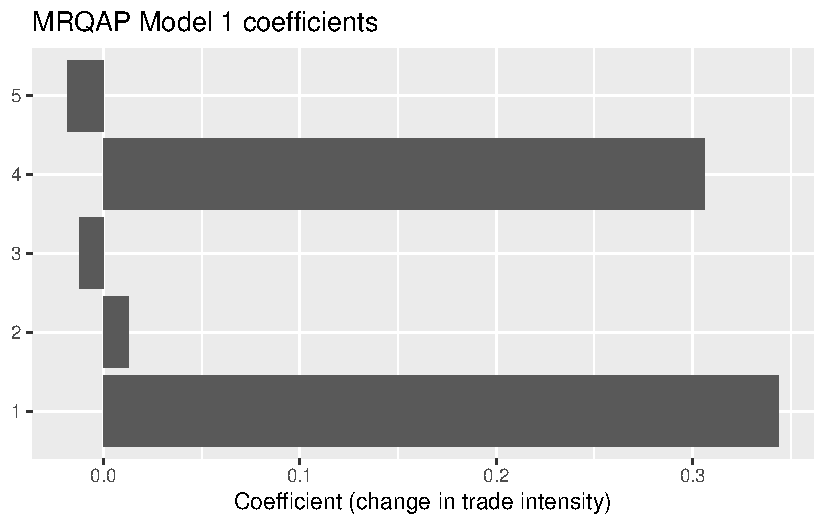
\includegraphics[keepaspectratio]{Report-Group-08-Quarto_files/figure-pdf/fig-mrqap-coefs-1.pdf}}

}

\end{figure}%

\subsection{ERGM -- Result for Research Question
2}\label{ergm-result-for-research-question-2}

To address our hypothesis, we constructed the final model using a set of
ERGM terms, which are defined in Table \ref{tbl_terms_testing}.

\begin{longtable}{p{10cm} p{4cm}}
\caption{ERGM Terms and Testing Overview}
 \\
\toprule
\textbf{ERGM Terms} & \textbf{Testing} \\
\midrule
\endhead

\midrule
\multicolumn{2}{r}{\footnotesize\emph{Continued on next page}} \\
\endfoot

\bottomrule
\endlastfoot

absdiff("regulatory\_quality") & Hypothesis H2a \\
absdiff("rule\_of\_law")  & Hypothesis H2b \\
mutual & Hypothesis H2c \\
dgwesp(decay = 0.025, fixed =TRUE, type="OTP") & Hypothesis H2d \\
nodeicov("log\_total\_imports") & Hypothesis H2e \\
gwidegree(0.025, fixed = TRUE) & Control variable \\
nodecov("gdp\_growth") & Control variable \\
dgwdsp(decay = 0.025, fixed =TRUE, type="OTP") & Control variable \\

\end{longtable}

Comparing the two model specifications (Table
\ref{tbl_ergm_comparison}), based on different binarisation thresholds
(top 10\% vs.~top 25\% of trade values), shows clear differences in
performance. Using standard fit measures, Model 2 (threshold 0.9)
performs substantially better than Model 1 (threshold 0.75), with much
lower AIC and BIC values. This suggests the strongest export ties follow
more systematic and predictable patterns. Once reciprocity, clustering,
popularity, and country characteristics are included, high-value export
relationships become highly structured. In contrast, relaxing the
threshold in Model 1 introduces more medium-intensity trade, which
creates greater variability and makes the results less clearly explained
by the same mechanisms. Overall, the most intense export links follow
stronger network rules than weaker or moderate ties.

From the non-structural perspective, both models shows a consistent
message. Countries with higher overall import volume are much more
likely to be the recipients of strong export ties in both models. This
effect is large and highly significant in both models (with coefficients
≈0.44 and 0.55), which directly supports H2e: large import markets act
as trade magnets and attract a large share of strong export
relationships. We also find that countries with more similar regulatory
quality are slightly more likely to share a strong export tie, which is
consistent with H2a, although the magnitude is modest compared with
import volume and the structural effects. By contrast, similarity in
rule-of-law conditions does not exhibit a robust pattern across models,
so we do not find support for H2b in this static 2018 snapshot. Finally,
higher GDP growth of exporters is associated with a minimal reduction in
the probability of sending strong ties (coefficients around −0.01 to
−0.02). Although statistically significant, this effect remains
substantively minor relative to import volume and the structural terms.

The structural terms are very stable across Model 1 and Model 2 and
strongly support H2c, H2d and H2e.First, reciprocity is extremely strong
(with coefficients ≈3.14 and 3.61): export relationships are far more
likely to be mutual than one-sided, supporting H2c and matching the idea
that strong trade ties usually reflect mutual economic dependence and
negotiated agreements rather than purely unilateral flows. Second, we
find clear evidence of clustering and triadic closure: A positive
coefficient of transitivity term (dgwesp.OTP) implies that countries
that share trading partners are much more likely to also trade strongly
with each other. This is the mechanism behind H2d and aligns with the
presence of regional blocs and tightly knit trade clusters, where
``partners of my partners'' tend to become my partners as well. Third,
the popularity effect, shown through the positive geometrically weighted
in-degree term, appears in both models: countries that already receive
many export ties are especially likely to attract additional exporters.
This reinforces hub-like structures in the network and, together with
the strong effect of being a large importer, provides further support
for H2e.

\begin{longtable}{p{4.5cm}| *{3}{>{\centering\arraybackslash}p{1.6cm}} | *{3}{>{\centering\arraybackslash}p{1.6cm}}}
\caption{Comparison of ERGM Results for Trade Networks (Thresholds 75\% and 90\%)} 
 \\
\hline
\multicolumn{1}{p{4.5cm}|}{Term} &
\multicolumn{3}{c|}{Model Threshold 0.75} &
\multicolumn{3}{c}{Model Threshold 0.90} \\
\cline{2-4} \cline{5-7}
& Estimate & Std. Error & \multicolumn{1}{c|}{Signif.} & Estimate & Std. Error & Signif. \\
\hline
\endhead
%
\hline
\multicolumn{7}{r}{\footnotesize\emph{Continued on next page}} \\
\endfoot
%
\hline
\multicolumn{7}{p{\linewidth}}{\footnotesize\emph{Note}: GW = geometrically weighted; OTP = outgoing two-paths; Signif. codes: p < 0.001 '***', p < 0.01 '**', p < 0.05 '*', p < 0.1 '.'} \\
\endlastfoot
%
Edges                          & -13.863 & 0.360 & *** & -15.646 & 0.418 & *** \\
Regulatory Quality (absdiff)  & -0.112 & 0.032 & *** & -0.210 & 0.044 & *** \\
Rule of Law (absdiff)         & 0.024  & 0.032 &     & -0.009 & 0.043 &     \\
Log Total Imports (nodeicov)   & 0.438  & 0.010 & *** & 0.554  & 0.018 & *** \\
GDP Growth                     & -0.011 & 0.004 & **  & -0.015 & 0.005 & **  \\
Mutual                         & 3.139  & 0.050 & *** & 3.609  & 0.077 & *** \\
Import popularity (gwideg)  & 3.839  & 0.313 & *** & 2.883  & 0.278 & *** \\
Transitivity effect (dgwesp.OTP) & 4.003  & 0.280 & *** & 3.286  & 0.202 & *** \\
Dyadwise shared partners (gwdsp.OTP)        & -0.108 & 0.003 & *** & -0.081 & 0.004 & *** \\
\hline
\textbf{AIC} & \multicolumn{3}{c|}{16117} & \multicolumn{3}{c}{8930} \\
\textbf{BIC} & \multicolumn{3}{c|}{16193} & \multicolumn{3}{c}{9005} \\
\end{longtable}

Compared with the earlier MRQAP analysis, the ERGM results provide a
more nuanced view. While MRQAP attributed most variation in trade
intensity to economic fundamentals---especially market size---and found
only a weak role for governance, the ERGM confirms those fundamentals
and adds that network structure itself is central: reciprocity,
clustering, and the prominence of major import hubs help explain which
country pairs trade most intensely. This echoes findings by (Gutierrez
et al., 2020), which identifies key structural drivers such as
reciprocity and economic scale in driving strong commodity flows.

On the other hand, the modest effect of governance similarity contrasts
with conclusions from where institutional quality and infrastructure
significantly influenced bilateral trade flows (Groot, Linders,
Rietveld, \& Subramanian, 2004). This suggests that while institutions
may matter for whether trade occurs at all, once strong ties exist,
network structure and economic scale dominate the intensity of those
ties. Ultimately, the 2018 export network appears highly reciprocal,
clustered, and hub-dominated, with large import markets and structural
network dynamics exerting far more influence on strong export
relationships than governance similarity. In this static view we
therefore find strong support for H2c, H2d, and H2e, partial support for
H2a, and no support for H2b.

The trace plots for both threshold specifications (Appendix
\ref{sec-mcmc-75}, Appendix \ref{sec-mcmc-90}) show stable and
well-mixed Markov chains, indicating successful convergence of the Monte
Carlo Maximum Likelihood Estimation (MCMLE) algorithm. The corresponding
density plots exhibit unimodal and regular distributions that are
centered around stable means, indicating consistent and robust parameter
estimation across iterations.

\subsubsection{Goodness of Fit}\label{goodness-of-fit}

The results of the goodness of fit analysis of Model 1 (threshold 0.75)
and Model 2 (threshold 0.9) are provided in Figure \ref{fig-mod-75} and
Figure \ref{fig-mod-90}. For all included terms, the observed statistics
fall well within the boxplots of the simulated networks, so the models
are internally consistent. However, Model 1 captures the overall network
structure more closely than Model 2.

For in-degree and out-degree distributions, both models show poor fit at
the extreme with the sharp spike at degree 0. Model 1 roughly tracks the
observed distributions but still underestimates how many countries have
very few partners. This problem is stronger in Model 2, where the real
network has more peripheral countries and fewer highly connected hubs
than the model simulation predicts.

For minimum geodesic distance diagnostics, both models show a robust fit
for most distances; the observed values are consistently within the
simulated distributions. In contrast, edgewise shared partner
diagnostics reveal that both models struggle with predicting lower
numbers of shared partners, indicating that both models over-predict the
number of connections that complete triangles or clusters compared to
what is observed in the real data, with the mismatch again larger for
Model 2. This is due to using a higher threshold: keeping only the top
10\% of trade ties produces an extremely sparse network where ties are
concentrated among only the strongest partners. The ERGM models, using
relatively generic terms, struggles to replicate this high concentration
of ties in hubs and the corresponding large number of completely
isolated (peripheral).The 25\% threshold network is denser and more
``average'' in its structure, making it a closer match to the general
distributions that standard ERGM terms can approximate.

\begin{figure}[H]

\caption{\label{fig-mod-75}The Goodness of Fit in the stimulated
networks with threshold 0.75. The minimum geodesic distance, in degree,
out degree and edge-wise shared partners are captured}

\centering{

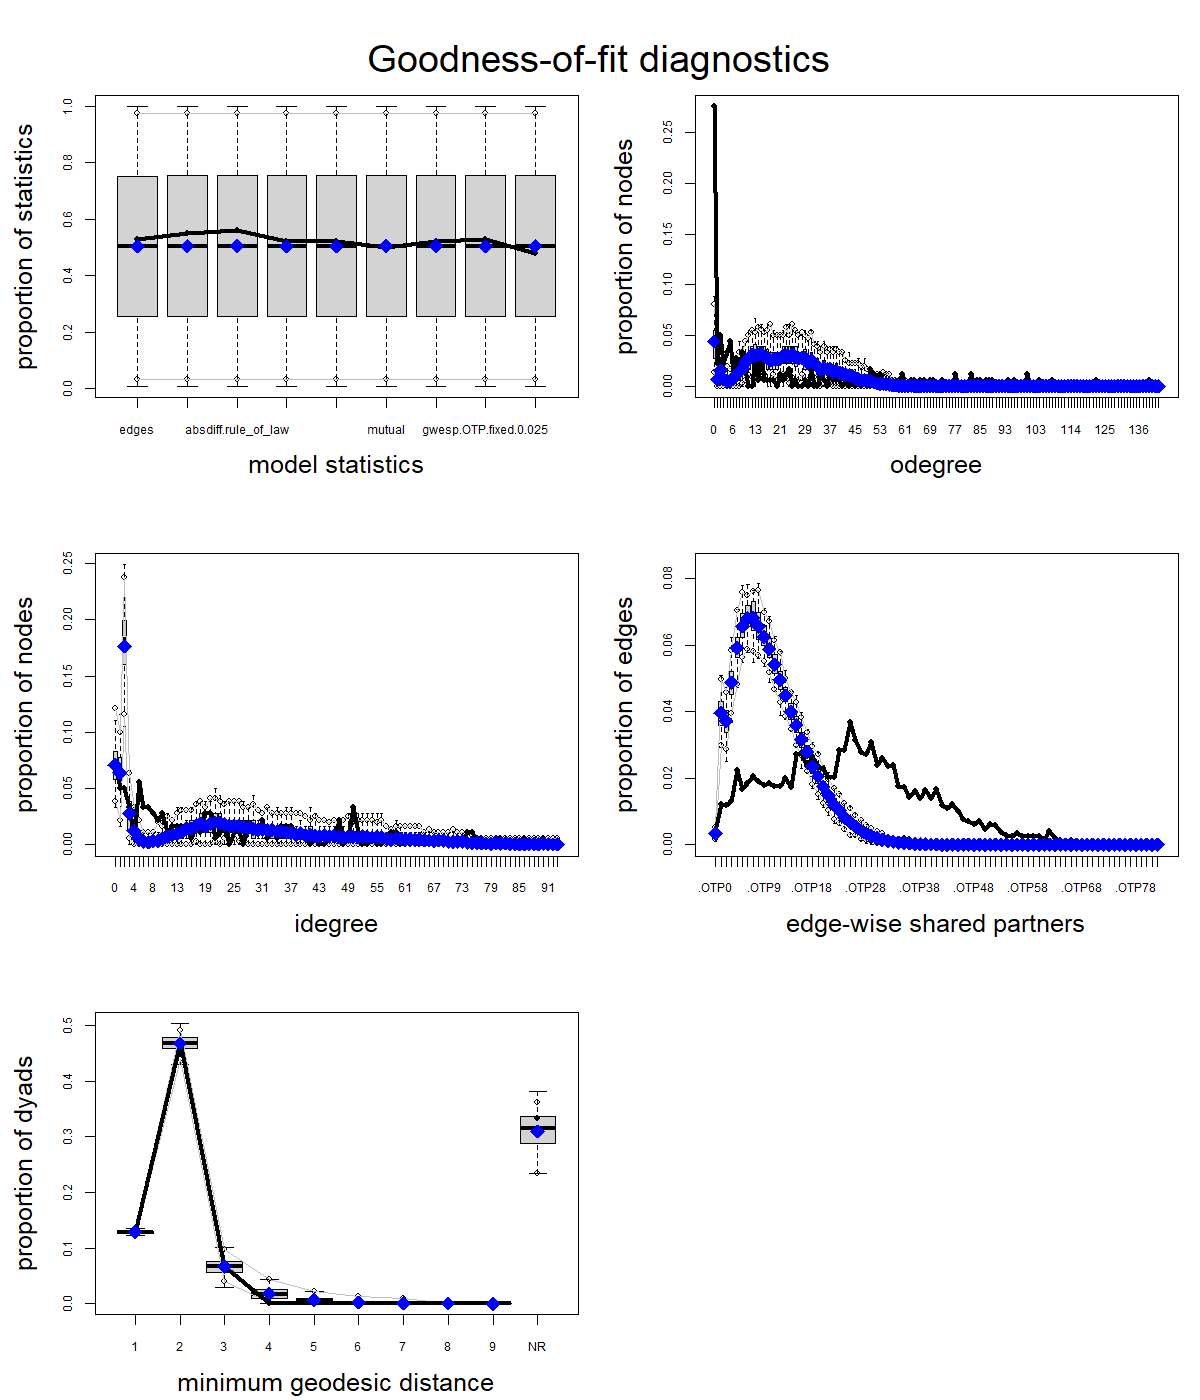
\includegraphics[width=0.85\linewidth,height=\textheight,keepaspectratio]{figures/gof_combined_plot_75.png}

}

\end{figure}%

\begin{figure}[H]

\caption{\label{fig-mod-90}The Goodness of Fit in the stimulated
networks with threshold 0.9. The minimum geodesic distance, in degree,
out degree and edge-wise shared partners are captured}

\centering{

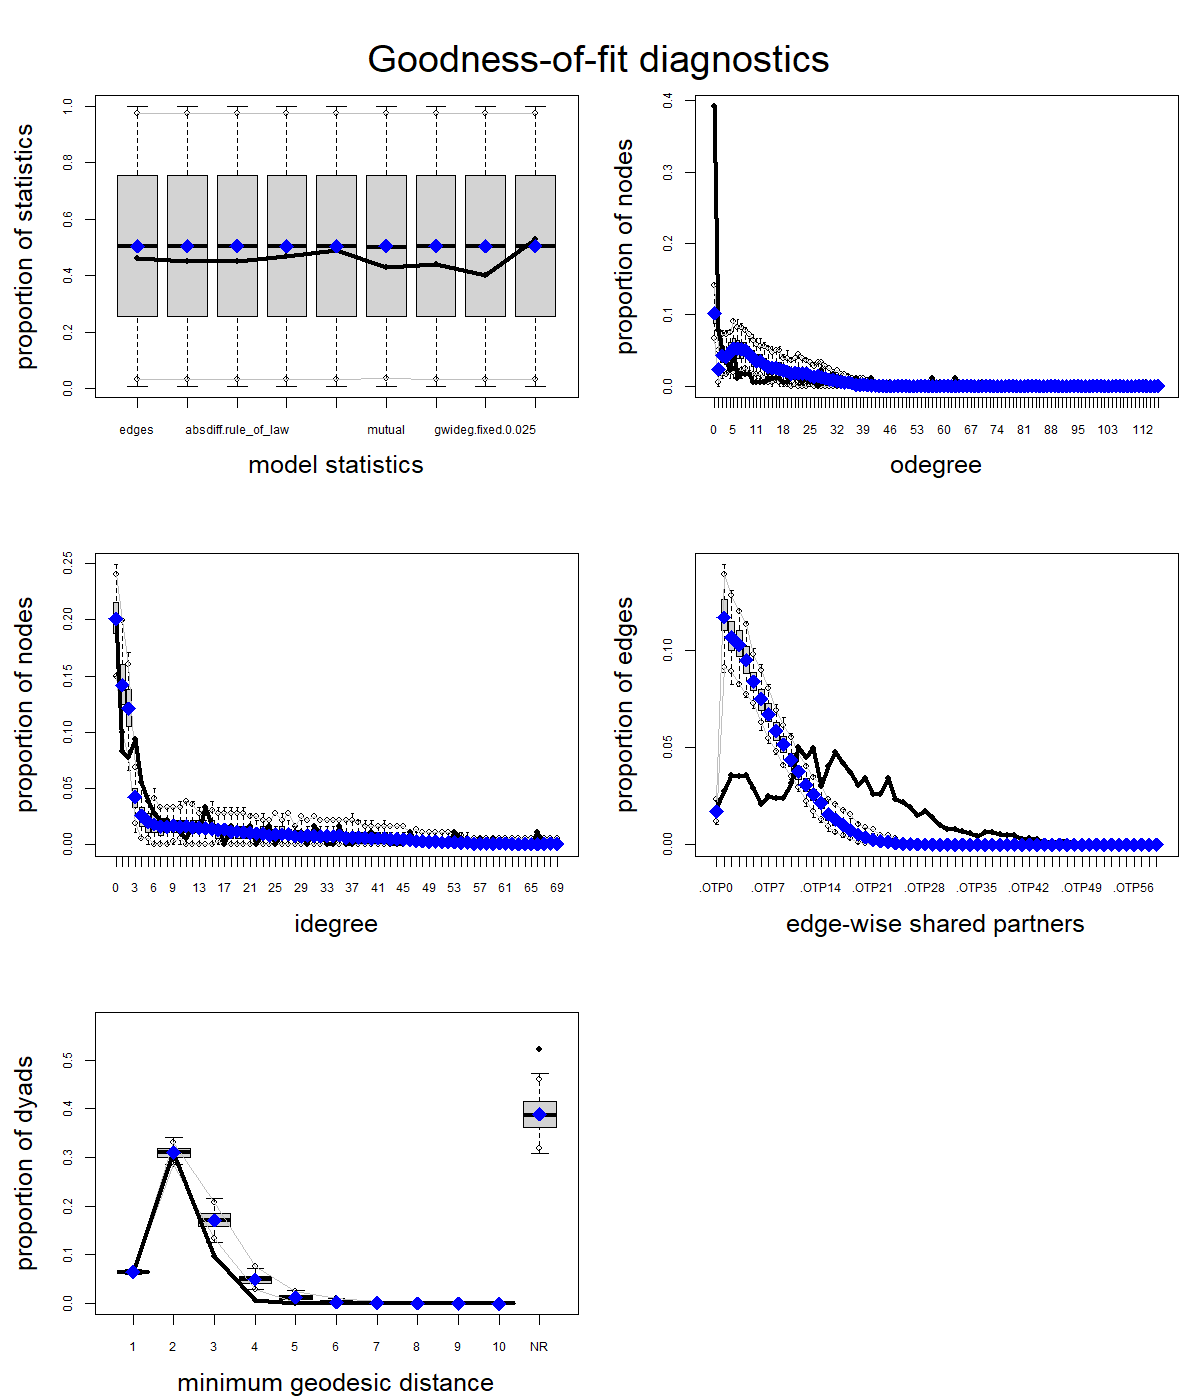
\includegraphics[width=0.85\linewidth,height=\textheight,keepaspectratio]{figures/gof_combined_plot_90.png}

}

\end{figure}%

\section{Conclusion}\label{conclusion}

\begin{itemize}
\item
  What were your topic and research questions again? 1 sentence only

  What did you learn from the two analyses you run? Most important point
  to address 0.5 POINTS
\item
  Who benefits from your findings?
\item
  What remains an open problem?
\item
  Can you give suggestions for future work in this area?
\end{itemize}

\section{References}\label{references}

\phantomsection\label{refs}
\begin{CSLReferences}{1}{0}
\bibitem[\citeproctext]{ref-noauthor_inferential_nodate}
Cranmer, S. J., \& Desmarais, B. A. (2011). Inferential {Network}
{Analysis} with {Exponential} {Random} {Graph} {Models} {\textbar}
{Political} {Analysis} {\textbar} {Cambridge} {Core}.
\url{https://doi.org/10.1093/pan/mpq037}

\bibitem[\citeproctext]{ref-de_groot_institutional_2004}
De Groot, H. L. F., Linders, G.-J., Rietveld, P., \& Subramanian, U.
(2004). The {Institutional} {Determinants} of {Bilateral} {Trade}
{Patterns}. \emph{Kyklos}, \emph{57}(1), 103--123.
\url{https://doi.org/10.1111/j.0023-5962.2004.00245.x}

\bibitem[\citeproctext]{ref-noauthor_sensitivity_nodate}
Dekker, D., Krackhardt, D., \& Snijders, T. (2007). Sensitivity of MRQAP
tests to collinearity and autocorrelation conditions.
\url{https://doi.org/10.1007/s11336-007-9016-1}

\bibitem[\citeproctext]{ref-desmarais_statistical_2012}
Desmarais, B. A., \& Cranmer, S. J. (2012). Statistical inference for
valued-edge networks: The generalized exponential random graph model.
\emph{PloS One}, \emph{7}(1), e30136.
\url{https://doi.org/10.1371/journal.pone.0030136}

\bibitem[\citeproctext]{ref-didier_characterising_2021}
Didier, L., \& Hoarau, J.-F. (2021). Characterising {Bilateral} {Trade}
between sub-{Saharan} {Africa} and {China}: {The} {Specific} {Role} of
{Institutional} {Quality}. \emph{Revue d'économie Politique},
\emph{131}(1), 57--88. \url{https://doi.org/10.3917/redp.311.0063}

\bibitem[\citeproctext]{ref-dixit_lawlessness_2011}
Dixit, A. (2011). Lawlessness and {Economics}: {Alternative} {Modes} of
{Governance}. \emph{Lawlessness and Economics: Alternative Modes of
Governance}.

\bibitem[\citeproctext]{ref-fagiolo_international-trade_2009}
Fagiolo, G. (2009). \emph{The {International}-{Trade} {Network}:
{Gravity} {Equations} and {Topological} {Properties}}. arXiv.
\url{https://doi.org/10.48550/arXiv.0908.2086}

\bibitem[\citeproctext]{ref-feng_service_2021}
Feng, L., Xu, H., Wu, G., \& Zhang, W. (2021). Service trade network
structure and its determinants in the {Belt} and {Road} based on the
temporal exponential random graph model. \emph{Pacific Economic Review},
\emph{26}(5), 617--650. \url{https://doi.org/10.1111/1468-0106.12378}

\bibitem[\citeproctext]{ref-francois_institutions_2013}
Francois, J., \& Manchin, M. (2013). Institutions, {Infrastructure}, and
{Trade}. \emph{World Development}, \emph{46}, 165--175.
\url{https://doi.org/10.1016/j.worlddev.2013.02.009}

\bibitem[\citeproctext]{ref-noauthor_pdf_2025-1}
Frankel, J., Wei, S.-J., \& Stein, E. (1995). Trading blocs and the
americas: The natural, the unnatural, and the super-natural.
\emph{Journal of Development Economics}, \emph{47}, 61--95.
\url{https://doi.org/10.1016/0304-3878(95)00005-4}

\bibitem[\citeproctext]{ref-de_groot_institutional_2004-1}
Groot, H. L. F. de, Linders, G.-J., Rietveld, P., \& Subramanian, U.
(2004). The {Institutional} {Determinants} of {Bilateral} {Trade}
{Patterns}. \emph{Kyklos}, \emph{57}, 103--123.
\url{https://doi.org/10.2139/ssrn.417323}

\bibitem[\citeproctext]{ref-noauthor_analysis_nodate}
Gutierrez, E., Adenso-Díaz, B., \& Lozano, S. (2020). Analysis and
vulnerability of the international wheat trade network {\textbar} {Food}
{Security}. \url{https://doi.org/10.1007/s12571-020-01117-9}

\bibitem[\citeproctext]{ref-horn_beyond_2010}
Horn, H., Mavroidis, P. C., \& Sapir, A. (2010). Beyond the {WTO}? {An}
{Anatomy} of {EU} and {US} {Preferential} {Trade} {Agreements}.
\emph{The World Economy}, \emph{33}(11), 1565--1588.
\url{https://doi.org/10.1111/j.1467-9701.2010.01273.x}

\bibitem[\citeproctext]{ref-hu_impacts_2023}
Hu, X., Sun, B., Wang, C., Lim, M. K., Wang, P., Geng, X., \ldots{}
Chen, W.-Q. (2023). Impacts of {China}'s exports decline in rare earth
primary materials from a trade network-based perspective.
\emph{Resources Policy}, \emph{81}.
\url{https://doi.org/10.1016/j.resourpol.2023.103321}

\bibitem[\citeproctext]{ref-landry_does_2024}
Landry, D. (2024). \emph{Does governance matter? {Comparing} the
determinants of {Chinese} and {Western} trade with {Africa}}. Retrieved
from \url{https://hdl.handle.net/10161/33504}

\bibitem[\citeproctext]{ref-leitao_gravity_2024}
Leitão, N. C. (2024). Gravity {Model} and {International} {Trade}: {A}
{Survey} of the {Literature}. \emph{Administrative Sciences},
\emph{14}(9), 219. \url{https://doi.org/10.3390/admsci14090219}

\bibitem[\citeproctext]{ref-noauthor_role_nodate}
Long, N., Gam, N., Vu Hong, V., \& Bui Hoang, N. (2023). The role of
cultural and institutional distances in international trade.
\url{https://doi.org/10.28991/ESJ-2023-07-02-015}

\bibitem[\citeproctext]{ref-noauthor_make_nodate}
Philippe, M., Thierry, M., \& Mathias, T. (2008). \emph{Make {Trade}
{Not} {War}? {\textbar} {The} {Review} of {Economic} {Studies}
{\textbar} {Oxford} {Academic}}. Retrieved from
\url{https://academic.oup.com/restud/article-abstract/75/3/865/1555305?redirectedFrom=fulltext}

\bibitem[\citeproctext]{ref-sabry_arab-german_2022}
Sabry, M. I. (2022). Arab-{German} {Trade} and {Institutions}: {The}
{Effect} of {Good} {Governance} on {Arab} {Exports} to {Germany}.
\emph{The European Journal of Development Research}, \emph{34}(5),
2400--2437. \url{https://doi.org/10.1057/s41287-021-00462-5}

\bibitem[\citeproctext]{ref-schweitzer_economic_2009}
Schweitzer, F., Fagiolo, G., Sornette, D., Vega-Redondo, F., Vespignani,
A., \& White, D. R. (2009). Economic networks: The new challenges.
\emph{Science (New York, N.Y.)}, \emph{325}(5939), 422--425.
\url{https://doi.org/10.1126/science.1173644}

\bibitem[\citeproctext]{ref-serrano_extracting_2009}
Serrano, M. A., Boguna, M., \& Vespignani, A. (2009). Extracting the
multiscale backbone of complex weighted networks. \emph{Proceedings of
the National Academy of Sciences}, \emph{106}(16), 6483--6488.
\url{https://doi.org/10.1073/pnas.0808904106}

\bibitem[\citeproctext]{ref-setayesh_analysis_2022}
Setayesh, A., Sourati Hassan Zadeh, Z., \& Bahrak, B. (2022). Analysis
of the global trade network using exponential random graph models.
\emph{Applied Network Science}, \emph{7}(1), 38.
\url{https://doi.org/10.1007/s41109-022-00479-7}

\bibitem[\citeproctext]{ref-shleifer_corruption_1993}
Shleifer, A., \& Vishny, R. W. (1993). Corruption*. \emph{The Quarterly
Journal of Economics}, \emph{108}(3), 599--617.
\url{https://doi.org/10.2307/2118402}

\bibitem[\citeproctext]{ref-university_of_economic_studies_bucharest_romania_governance_2021}
Tamas, A., \& Miron, D. (2021). The governance impact on the romanian
trade flows. An augmented gravity model.
\emph{Www.amfiteatrueconomic.ro}, \emph{23}, 276.
\url{https://doi.org/10.24818/EA/2021/56/276}

\bibitem[\citeproctext]{ref-uncomtrade_2025}
UN Comtrade. (2025). \emph{{UN Comtrade Database}}.
\url{https://comtradeplus.un.org/}.

\bibitem[\citeproctext]{ref-worldbank_dbi_2020}
World Bank. (2020). \emph{Doing business database}.
\url{https://databank.worldbank.org/source/doing-business}.

\bibitem[\citeproctext]{ref-worldbank_wgi_2024}
World Bank. (2024). \emph{Worldwide governance indicators}.
\url{https://databank.worldbank.org/source/worldwide-governance-indicators}.

\bibitem[\citeproctext]{ref-worldbank_wdi_2025}
World Bank. (2025). \emph{World development indicators}.
\url{https://databank.worldbank.org/source/world-development-indicators}.

\bibitem[\citeproctext]{ref-noauthor_structural_nodate}
Yang, L., Shen, N., Szakálné Kanó, I., Kosztopulosz, A., \& Hu, J.
(2025). Structural evolution and factors of the electric vehicle
lithium-ion battery trade network among european union member states.
\url{https://doi.org/10.3390/su17156675}

\end{CSLReferences}

\section{Appendix}\label{appendix}

\subsection{Appendix A: MCMC Diagnostics of ERGM model applying 0.75
threshold}\label{sec-mcmc-75}

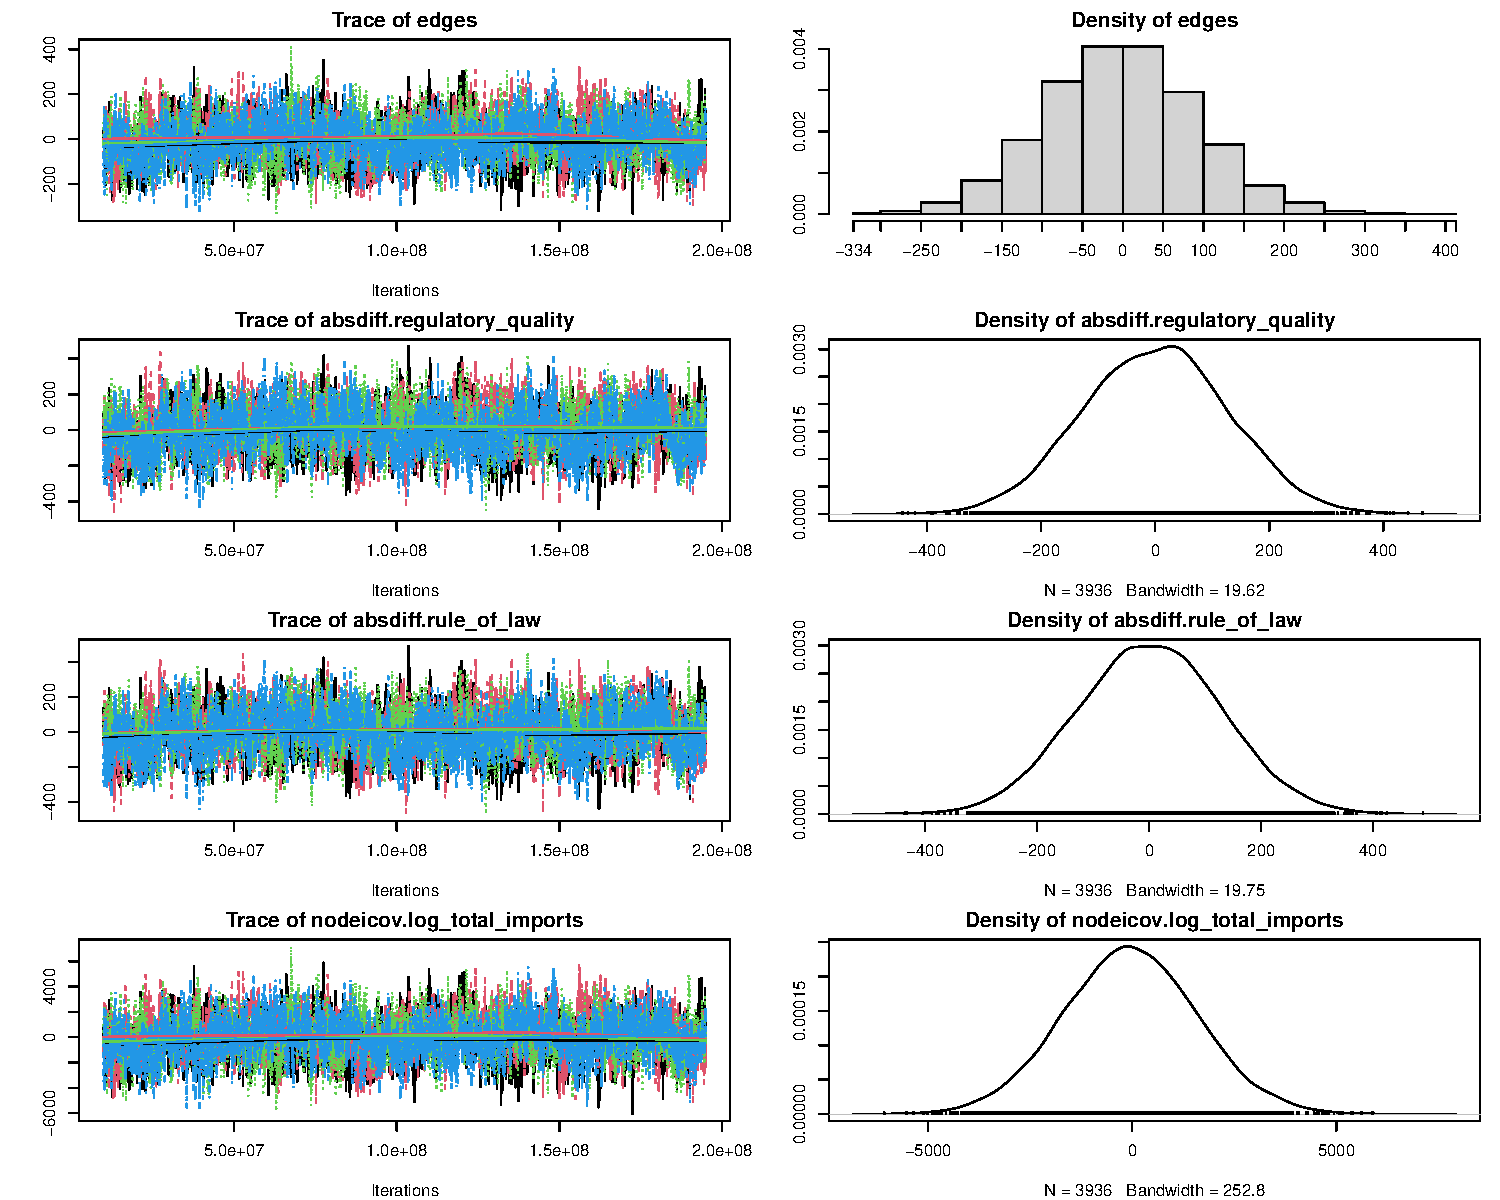
\includegraphics[width=0.75\linewidth,height=\textheight,keepaspectratio,page=1]{figures/mcmc_diagnostics_mod75.pdf}

\includegraphics[width=0.75\linewidth,height=\textheight,keepaspectratio,page=2]{figures/mcmc_diagnostics_mod75.pdf}

\includegraphics[width=0.75\linewidth,height=\textheight,keepaspectratio,page=3]{figures/mcmc_diagnostics_mod75.pdf}

\newpage{}

\subsection{Appendix B: MCMC Diagnostics of ERGM model applying 0.9
threshold}\label{sec-mcmc-90}

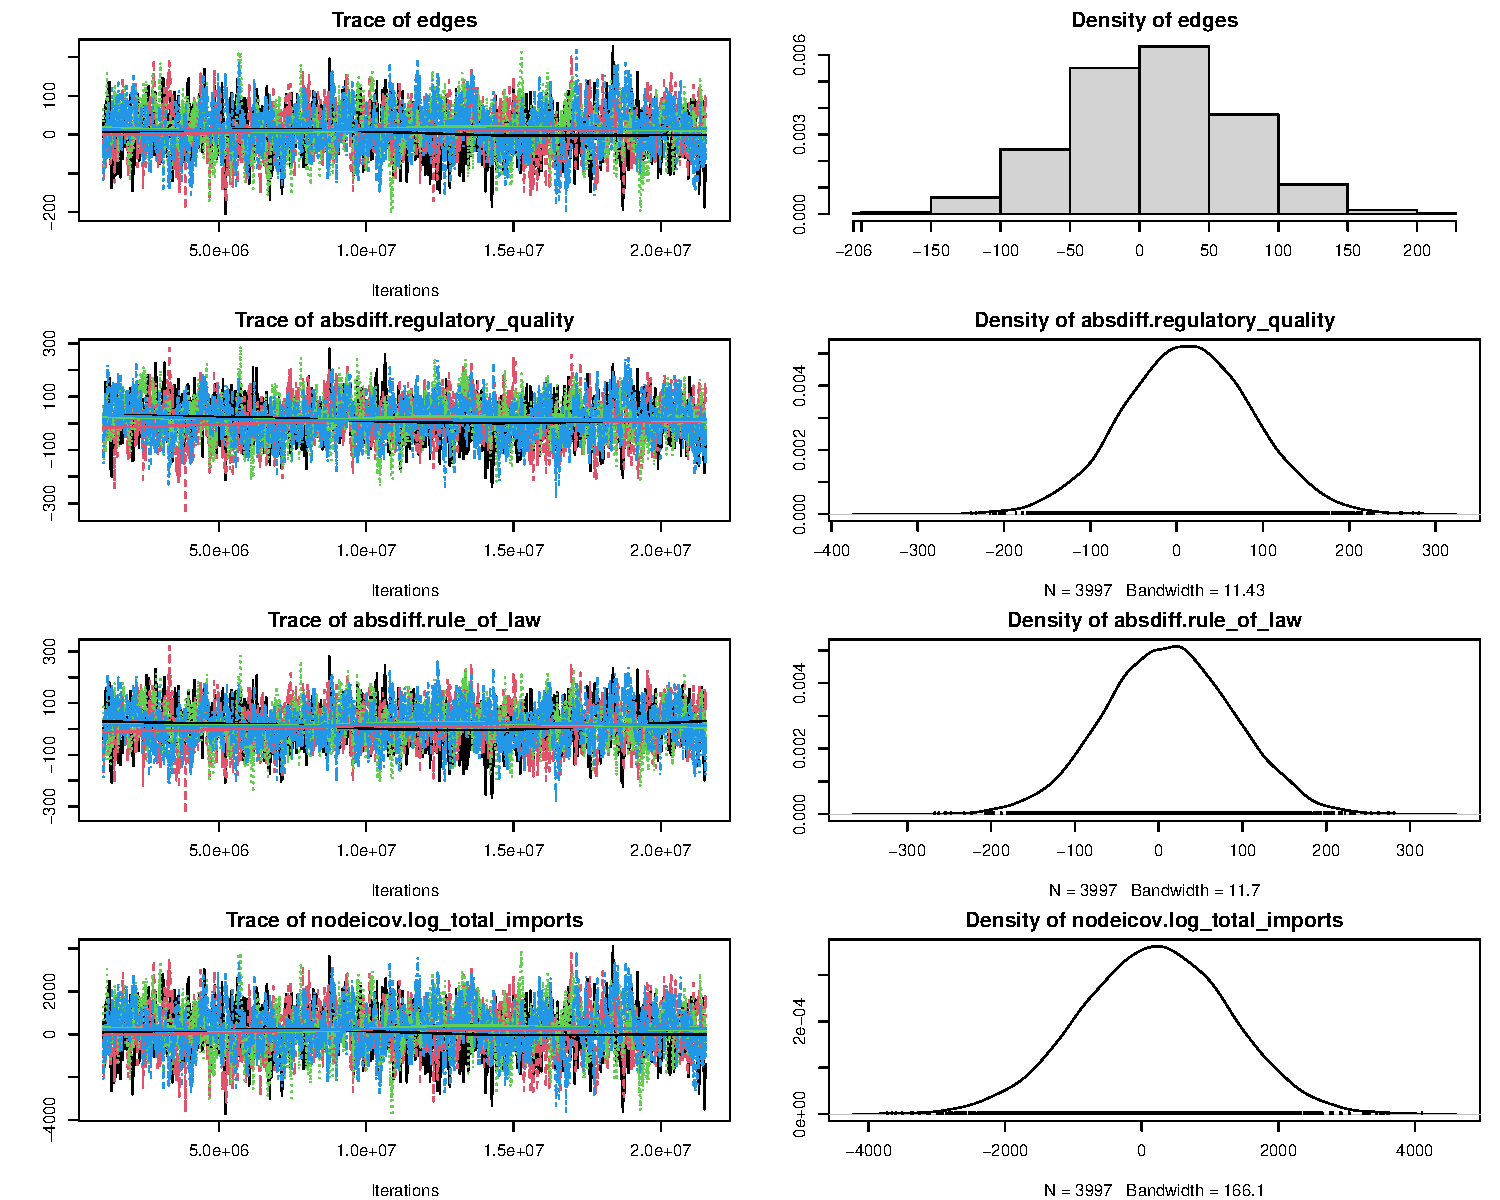
\includegraphics[width=0.75\linewidth,height=\textheight,keepaspectratio,page=1]{figures/mcmc_diagnostics_mod90.pdf}

\includegraphics[width=0.75\linewidth,height=\textheight,keepaspectratio,page=2]{figures/mcmc_diagnostics_mod90.pdf}

\includegraphics[width=0.75\linewidth,height=\textheight,keepaspectratio,page=3]{figures/mcmc_diagnostics_mod90.pdf}

\newpage{}

\section*{Technology statement}\label{technology-statement}
\addcontentsline{toc}{section}{Technology statement}

During the preparation of this work, we used \textbf{ChatGPT} to
\textbf{check spelling, grammar, coherence, syntax and support our
brainstorming process}. The sections affected by the use of this tool
include the \textbf{Introduction} and the \textbf{Research Rationale}.
All outputs generated by ChatGPT were critically reviewed, validated,
and edited by \textbf{Group 08 (Leon Boeren - Noud van Summeren - Chau
Nguyen - Paritosh Singh - Silvia Petrova)} to ensure accuracy and
academic integrity. \textbf{Group 08} assumes full responsibility for
the final content of this work.




\end{document}
